\documentclass[a4paper,english, 11pt]{article}


\usepackage[utf8]{inputenc}
\usepackage[T1]{fontenc}
\usepackage{lmodern} 
\usepackage[table]{xcolor}
\usepackage{parskip} 
\usepackage{amssymb,amsthm,framed}  
\usepackage[]{amsmath} 
\usepackage[hang,small,bf]{caption}
\usepackage{subcaption}
\usepackage{siunitx} 
\usepackage{bm}
\usepackage{url}  
\usepackage{multirow} 
\usepackage[hidelinks]{hyperref}
\usepackage[a4paper,inner=2.5cm,outer=2.5cm,top=2.5cm,bottom=2.5cm,pdftex]{geometry} 
\usepackage{array}
\usepackage{ragged2e}
\usepackage{fancyhdr}
\usepackage{tcolorbox}
\newcolumntype{P}[1]{>{\RaggedRight\hspace{0pt}}p{#1}}

\sisetup{product-units=single}

%  
\usepackage{listings}
\lstset{language=bash}
\lstset{basicstyle=\ttfamily,
  numbers=left,
  showstringspaces=false,
  commentstyle=\color{red},
  keywordstyle=\color{black},
  breaklines=true,
  belowskip=0.5em
}


\usepackage{accsupp}    
\lstset {
    numberstyle=\noncopynumber,
    columns=flexible,
}

\newcommand{\noncopynumber}[1]{
    \BeginAccSupp{method=escape,ActualText={}}
    #1
    \EndAccSupp{}
}


\usepackage{graphicx}     

\usepackage{enumitem}      
\graphicspath{{../Images/}} 
 
\hyphenpenalty=5000
\tolerance=1000
\title{The Nansen Legacy labelling manual}
\date{\today\\v0.4}
\author{Pål Ellingsen (\url{data.nleg@unis.no})}

\begin{document}
\maketitle
\tableofcontents
\pagestyle{fancy}
\newpage
\section{Introduction} % (fold) {{{
\label{sec:Introduction}

The Nansen Legacy project is aimed at generating samples, data and science relevant during the project and after its conclusion. Additionally it is a collaboration between major marine institutions in Norway. To accommodate the tracking of samples from ship to land and between institutions it was decided to use a unified labelling system. To secure that the project data and metadata follows the FAIR (Findable, Accessible, Interoperable, Reproducible) principle for data management within the project, a first step is to ensure that the collected samples are findable and that relevant metadata are logged
along with the sample collection. The metadata needs to be logged in a standardized manner and will be
made accessible through a search interphase as soon as possible after the cruises.  This manual details how to label samples, log the metadata and how to find information about logged samples in the SIOS database.  

% section Introduction (end) }}}


\subsection{Hierarchy} % (fold) {{{
\label{sub:Hirarcy}

One of the backbones of the sample log is the use of parent IDs. A parent ID is the ID of the gear cast or sample which a sample or sub-sample comes from, see figure~\ref{fig:parent_uuid}. By registering the parent, it is possible to keep track of which samples belong together, and any number of levels of sub-samples. Additionally it reduces the amount of information that needs to be registered on a sample, as information like for example position, bottom depth, date and time can be inherited from the parent. 
% subsection Hierarchy (end) }}}

\subsubsection{Overview webpage} % (fold) {{{
\label{ssub:Overview_webpage}

The overview webpage is where all of the tools and printing software on the cruise is located. It runs on the ship and is therefore available during the whole cruise, independent of Internet access. 
It can be found by opening a browser and going to the address \url{http://10.3.65.20}. What you should then see is something like what is shown in figure~\ref{fig:Printing_overview}.

\begin{figure}[htb]
    \tcbox[colback=white]{
    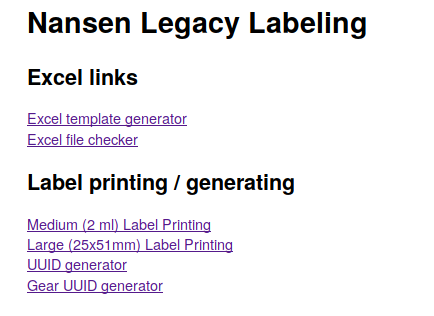
\includegraphics[width=0.6\textwidth]{Printing_overview.png}
    }
    \caption{\label{fig:Printing_overview}
        The overview webpage available on the ship.
    }
\end{figure}

% subsubsection Overview webpage (end) }}}

\begin{figure}[htbp]
    \centering
    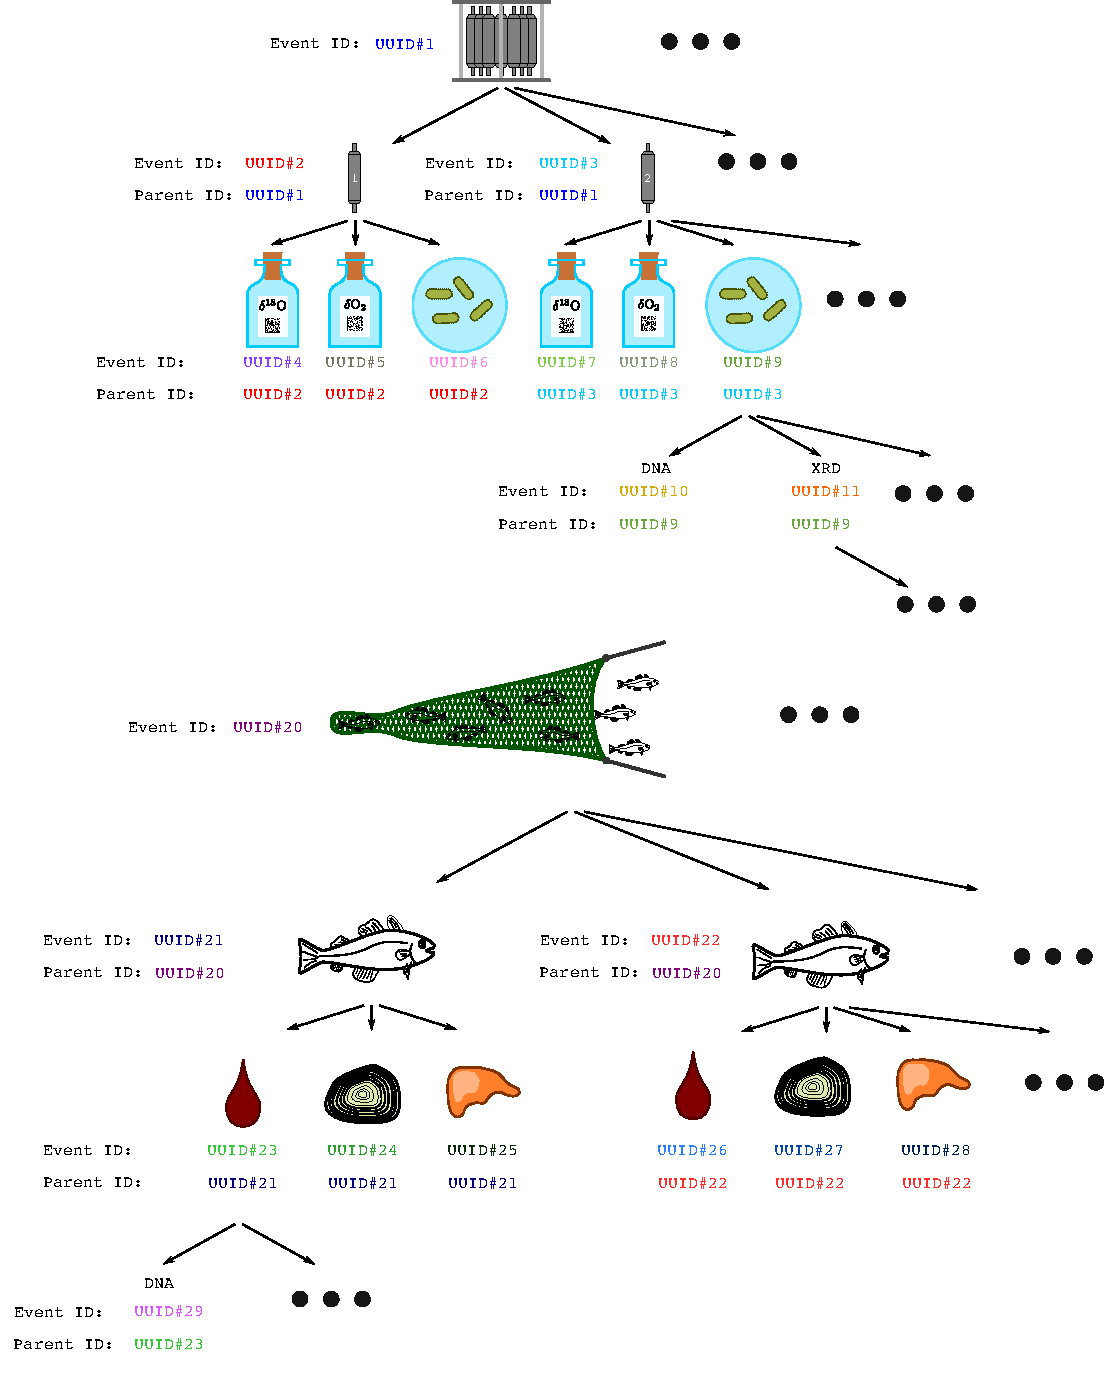
\includegraphics[width=1\textwidth]{Labeling.pdf}
    \caption{\label{fig:parent_uuid}
       Examples of how event id and parent id works for two different gear types. These should be transferable to other gear types.
    }
\end{figure}
\section{Labelling samples} % (fold) {{{
\label{sec:labelling samples}



In order to distinguish samples, samples in the project are assigned a unique id, in the form of a universally unique identifier (UUID). Details about it can be found in subsection~\ref{sub:UUID}. For physical samples this UUID is encoded in the form of a 2D barcode, specifically a Data Matrix (DM) code, details in subsection~\ref{ssub:DM}. An example of such a code can be seen in figure~\ref{fig:data_matrix}. The code is then printed, together with a descriptive text, onto a label which is stuck on the sample or its container.

\begin{figure}[htb]
    \centering
    
\includegraphics[width=0.1\textwidth]{Data_matrix.png}
    \caption{\label{fig:data_matrix}
        Example Data Matrix code containing an UUID.
    }

\end{figure}

\subsection{Procedure for physical samples} % (fold) {{{
\label{sub:Procedure for physical samples}


The interface for printing labels is available through a webpage on the research ship. Details of this is given by the cruise leader. Figure~\ref{fig:printing} shows how the two printing pages look.

\begin{enumerate}
    \item Choose label size.
    \item Write information which is to be printed together with the label into the printing page. This should include the date and information about what the sample is.
    \item Print the label.  
\end{enumerate}
The following steps can be done in any order depending on what is easiest:
\begin{enumerate}
\setcounter{enumi}{3}
    \item Stick the label on the sample
    \item Register data about the sample in the spreadsheet, see section~\ref{sub:spreadsheet_reg}.
\end{enumerate}

%\begin{figure}[h]
%% Uses the subcaption package
    %\centering
    %\begin{subfigure}[b]{0.49\textwidth}
        %\includegraphics[width=\textwidth]{Medium_print.png}
    %\end{subfigure}
    %\begin{subfigure}[b]{0.49\textwidth}
        %\includegraphics[width=\textwidth]{Large_print.png}
    %\end{subfigure}
    %\caption{\label{fig:printing}
    %Example of how the printing pages look.}
%\end{figure}
\begin{figure}[htb]
    \tcbox[colback=white]{
    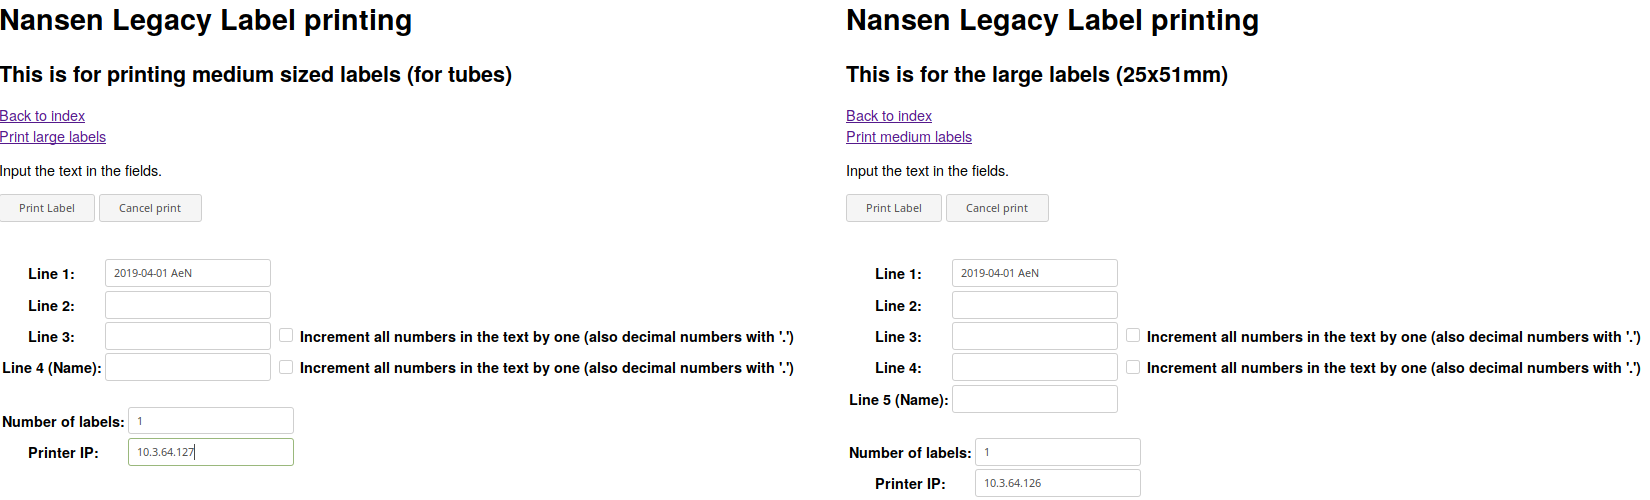
\includegraphics[width=1\textwidth]{Printing.png}
}
    \caption{\label{fig:printing}
        Two printing pages. Left the one for the medium sized labels and right for the large labels.
    }
\end{figure}

% subsection Procedure for physical samples (end) }}}

\subsection{Procedure for virtual samples} % (fold) {{{
\label{sub:Procedure_for_virtual_samples}



Examples of virtual sample are: gear casts, CTD Niskin bottles, Multicores, Multinets and Ice cores that have been split/melted. None of these samples have a physical/practical place for a label. They still need to be logged in the sample log (database), to ensure traceability of samples from them, see figure~\ref{fig:parent_uuid}. The procedure of logging them involves either printing a sheet of paper with codes or just assigning them a UUID without any Data Matrix code. Which approach is the best depends on the circumstance. These codes are then scanned/copied into the relevant sample log spreadsheet. If the UUID is going to be used by more than one scientist, for example in the case of Niskin bottles, it is often easier to print an A4 page with the codes. 

Below follows two different procedures depending on what is chosen:

\subsubsection{A4 page of codes} % (fold) {{{
\label{ssub:A4_page}

Go to the ''Gear UUID generator'' page on the printing overview (see subsection~\ref{ssub:Overview_webpage}). 
On this page you specify the name of the gear ''Gear Name'' (CTD, Multinet, Multicorer), the type of container ''Sample Name'' (Niskin, core, net), number of samples in one gear cast ''Number of samples'' and number of gear casts expected ''Number of pages'' (this is only to save having to come to this page for every cast). 

By pressing ''Make PDF'' a PDF is generated and can be printed on an normal printer. The A4 page printed should be marked with information identifying which gear cast this is for. Then all the containers need to be registered in the same way physical samples are, see subsection~\ref{sub:spreadsheet_reg}.

\textbf{Note: It is very important that one person is responsible for registering the containers, because without the container IDs , the samples will be without parents and untraceable.}

If copies are needed for several scientists to work on the same containers, the A4 page can be copied on a photocopier. 

\begin{figure}
% Uses the subcaption package
    \centering
    \begin{subfigure}[t]{0.45\textwidth}
        \vspace{0pt}
        \tcbox[colback=white]{
        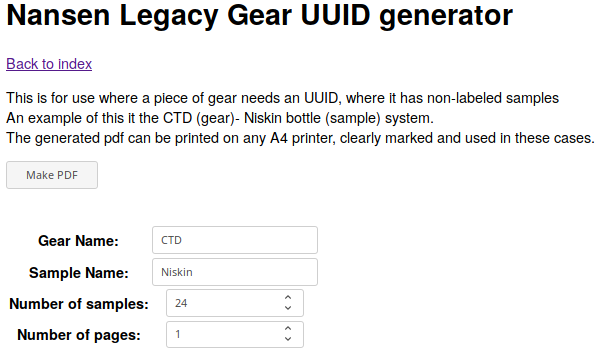
\includegraphics[width=\textwidth]{Gear_overview.png}
    }
    \end{subfigure}\hfill
    \begin{subfigure}[t]{0.47\textwidth}
        \vspace{0pt}
    \tcbox[colback=white]{
        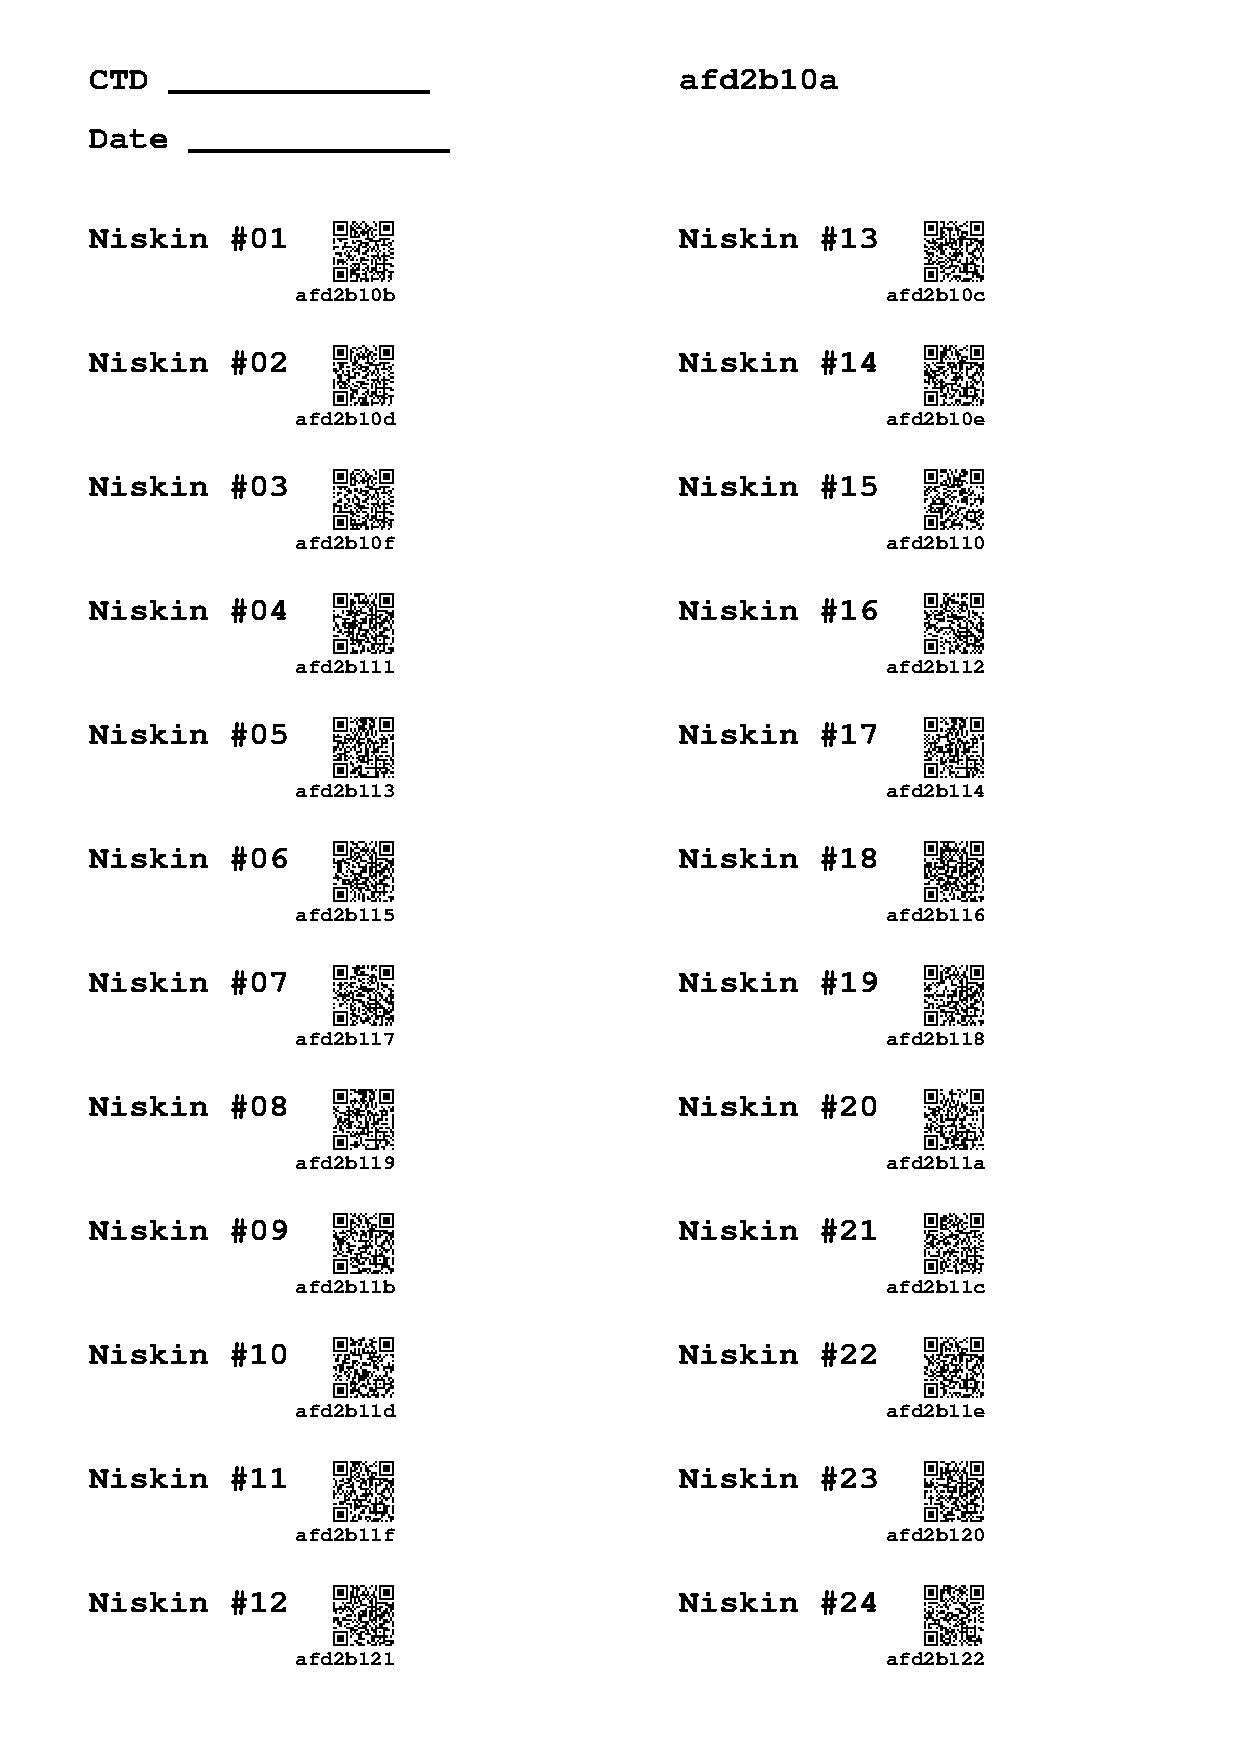
\includegraphics[width=\textwidth]{gear.pdf}
    }
    \end{subfigure}
    \caption{\label{fig:gear_overview}
        Left gear overview page and right an example output pdf file.
    }
\end{figure}
% subsubsection A4_page (end) }}}

\subsubsection{Only UUID} % (fold) {{{
\label{ssub:Only_UUID}

When only the UUID is needed, one can be generated through the ''UUID generator'' on the printing overview (subsection~\ref{ssub:Overview_webpage}), see figure~\ref{fig:uuid_gen}. Pick any one of the UUIDs and continue the registration as in subsection~\ref{sub:spreadsheet_reg}. In order to not reuse UUIDs, remember to use the ''Get new UUID'' button for every time you have used the displayed codes. A good procedure is to get new codes every time you go back to the page.

\begin{figure}[htb]
    \tcbox[colback=white]{
    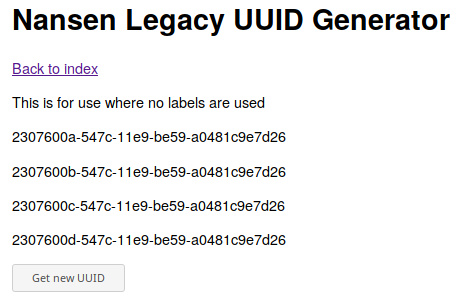
\includegraphics[width=0.5\textwidth]{UUID_gen.png}
}
    \caption{\label{fig:uuid_gen}
        UUID generator webpage.
    }
\end{figure}

% subsubsection Only_UUID (end) }}}
% subsection Procedure for virtual samples (end) }}}


\subsection{Generation of sample log spreadsheet} % (fold) {{{
\label{sub:Sample_log_spreadsheet_generation}

In order to log the samples labelled on a cruise, a standardised spreadsheet is used. The spreadsheet is based on Darwin Core. A generator for the spreadsheet can be found on the SIOS page (or on the ship), specifically at \url{https://www.sios-svalbard.org/cgi-bin/darwinsheet/?setup=aen}. When loading the page, certain parameters are already ticked, these are mandatory and should not be removed.  
The procedure is then to select the wanted columns and generate the sheet. \textbf{Each group (i.e. microbial, zooplankton, fish, chemistry, ...) should agree upon which columns are compulsory.} If a column is forgotten, a new sheet can be generated and the column copied into an existing spreadsheet.

When working with the spreadsheet the order of columns can be changed, but it is important to move the whole column as the third row contains the key used by the data manager to read the log into the database. 

It is possible to register information in the spreadsheet that does not appear in the final sample log, for instance a taxon classification you are unsure of, a calculation, ... By leaving the third row of the column empty, it will be ignored when the spreadsheet is read into the sample log. The same applies to rows with an empty event id.


% subsection   (end) }}}

\subsection{Sample logging} % (fold) {{{
\label{sub:spreadsheet_reg}


The samples taken during a cruise need to be logged in a standardised spreadsheet, see subsection~\ref{sub:Sample_log_spreadsheet_generation} for how to make one. Logging of samples should be done continuously during the cruise. 

When logging the sample you will need its id, for physical samples this id goes in the Sample ID field and should be entered by scanning the Data Matrix code on the sample label. Scanning the Data Matrix is done with a handheld scanner, see figure~\ref{fig:scanner}, that plugs into the USB port on your computer, available on the ship. When it is plugged in you should be able to place the marker in the event id field and push the button when the scanner is pointed at the sample label in question. 


\begin{figure}[h!tb]
    \centering
    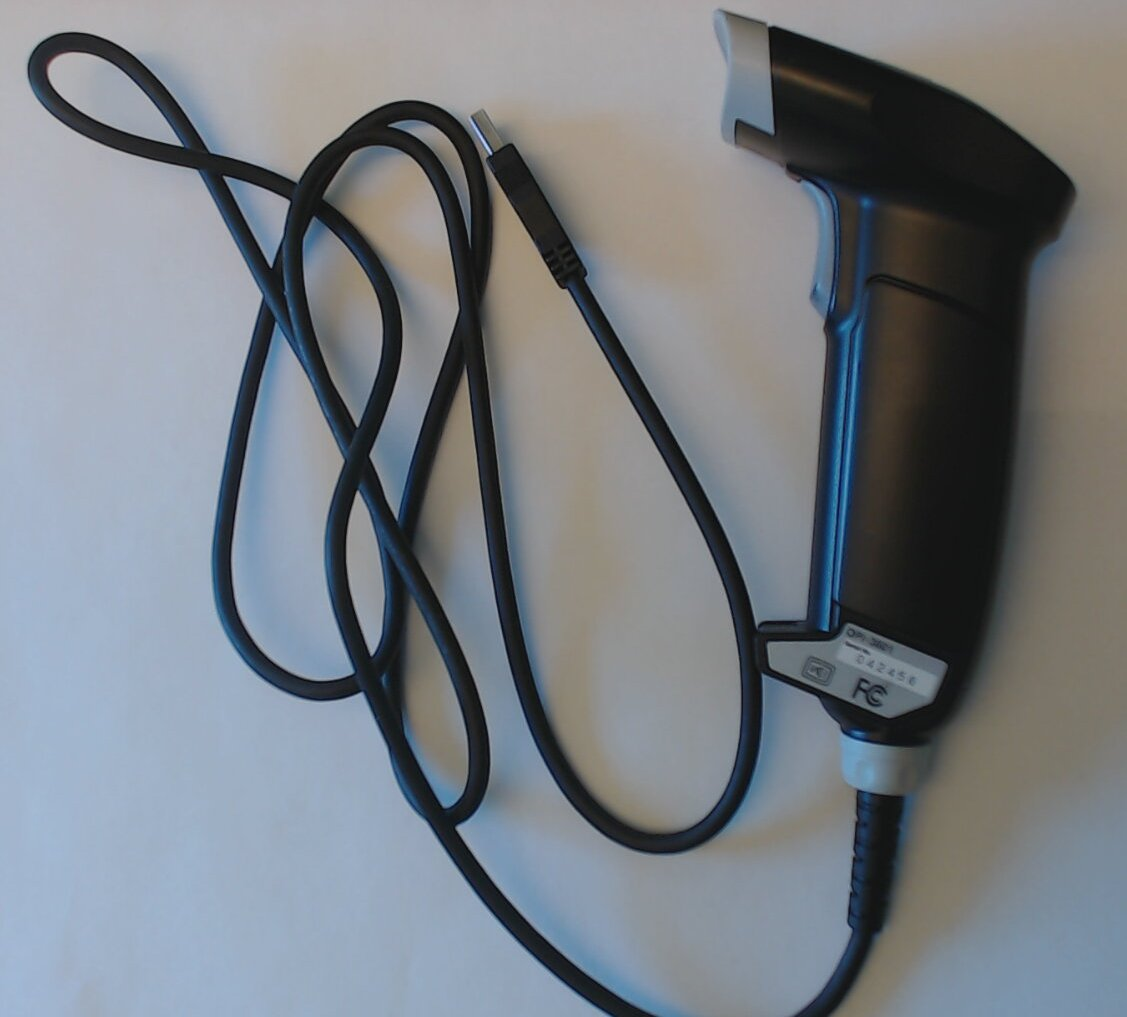
\includegraphics[width=0.3\textwidth]{Scanner.jpg}
    \caption{\label{fig:scanner}
        An Opticon OPI-3601 USB scanner.
    }
\end{figure}


Then its parent, see subsection~\ref{sub:Hirarcy}, needs to be registered, what the parent is depends on what type of sample it is, see figure~\ref{fig:parent_uuid} for some examples. Having registered these two, the rest of the columns in the spreadsheet need to be filled out. Every column has an explanation of what is expected in the given field. 

In order for the spreadsheet to be read into the sample log after the cruise, the spreadsheet needs to pass a format checker, see figure~\ref{fig:checker}, that checks all the entered fields for invalid and/or missing values. This checker is available on the ship through the overview page, see subsection~\ref{ssub:Overview_webpage}. It is \textbf{required} to run and pass this checker before uploading your spreadsheet to the data server on the ship at the end of the cruise. It is recommended to run this checker during the cruise, as errors can then easily be fixed.

\emph{Note that the sheet named ''Metadata'' needs to be filled out before running the checker.}

\begin{figure}[htb]
    \tcbox[colback=white]{
    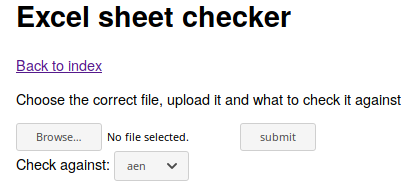
\includegraphics[width=0.45\textwidth]{Checker.png}
}
    \caption{\label{fig:checker}
        Excel spreadsheet checker. Should be on \emph{aen} for Nansen Legacy sample log.
    }
\end{figure}

% subsection Sample log spreadsheet logging (end) }}}

\subsection{End of cruise} % (fold) {{{
\label{sub:end_of_cruise}

At the end of the cruise, before going ashore, the finished spreadsheets need pass the checker routine, see subsection~\ref{sub:spreadsheet_reg}. After passing the checker, they should be stored with the official cruise data from the cruise. This is handled by the cruise leader and the IMR instrument responsible on the cruise. In addition to the sample spreadsheet, any collected data needs to be uploaded to the official cruise data.

% subsection end_of_cruise (end) }}}
\section{Label types} % (fold) {{{
\label{sub:Labels}

When selecting labels there are several considerations to be taken into account. Important considerations are which conditions will the labels be subject to and what type of container are they going on.

In the Nansen Legacy several different labels are available and can be printed on the Zebra label printers on the ship. Table~\ref{tab:labels} contains an overview of them and should be used to choose the appropriate one.

\begin{table}[htbp]
    \rowcolors{3}{cyan!10}{white}
    \caption{\label{tab:labels} An overview of different labels and their properties. All labels are waterproof and can withstand most laboratory chemicals}
    \begin{tabular}{l|P{3cm}lP{4cm}P{4cm}}
        \hline
        \textbf{Label} & \textbf{Size} & \textbf{Temp. range} & \textbf{Amount of text} & \textbf{Notes} \\ \hline
        Small& \SI{10}{\mm} diameter & \SIrange{-80}{135}{\celsius} & No text, only DM & Problems sticking on certain plastic bags in \SI{-20}{\celsius}\\
        Medium& \SI{19 x 25}{\mm}, fits Eppendorf \SI{2}{\ml} tubes & \SIrange{-196}{155}{\celsius} & 4 lines of 18 characters each & Problems sticking on certain plastic bags in \SI{-20}{\celsius}. \\
        Large& \SI{25 x 51}{\mm} & \SIrange{-80}{135}{\celsius} & 4 lines of 20 characters each, one with 36 characters. & Problems sticking on certain plastic bags in  \SI{-20}{\celsius}.\\
        \hline
    \end{tabular}
\end{table}





% section Marking samples (end) }}}

\section{Searching for samples} % (fold) {{{
\label{sec:Searching_sample}

If you want to find something in the sample log, there are several ways of searching it.
The sample log is located on the SIOS page, at \url{https://sios-svalbard.org/reports/aen_multi}.
On the page you will find a list of links under "Nansen Legacy Tools" in addition to links pointing to the sampling protocols, see figure~\ref{fig:sios}.

\begin{figure}[htb]
    \centering
    \tcbox[colback=white]{
    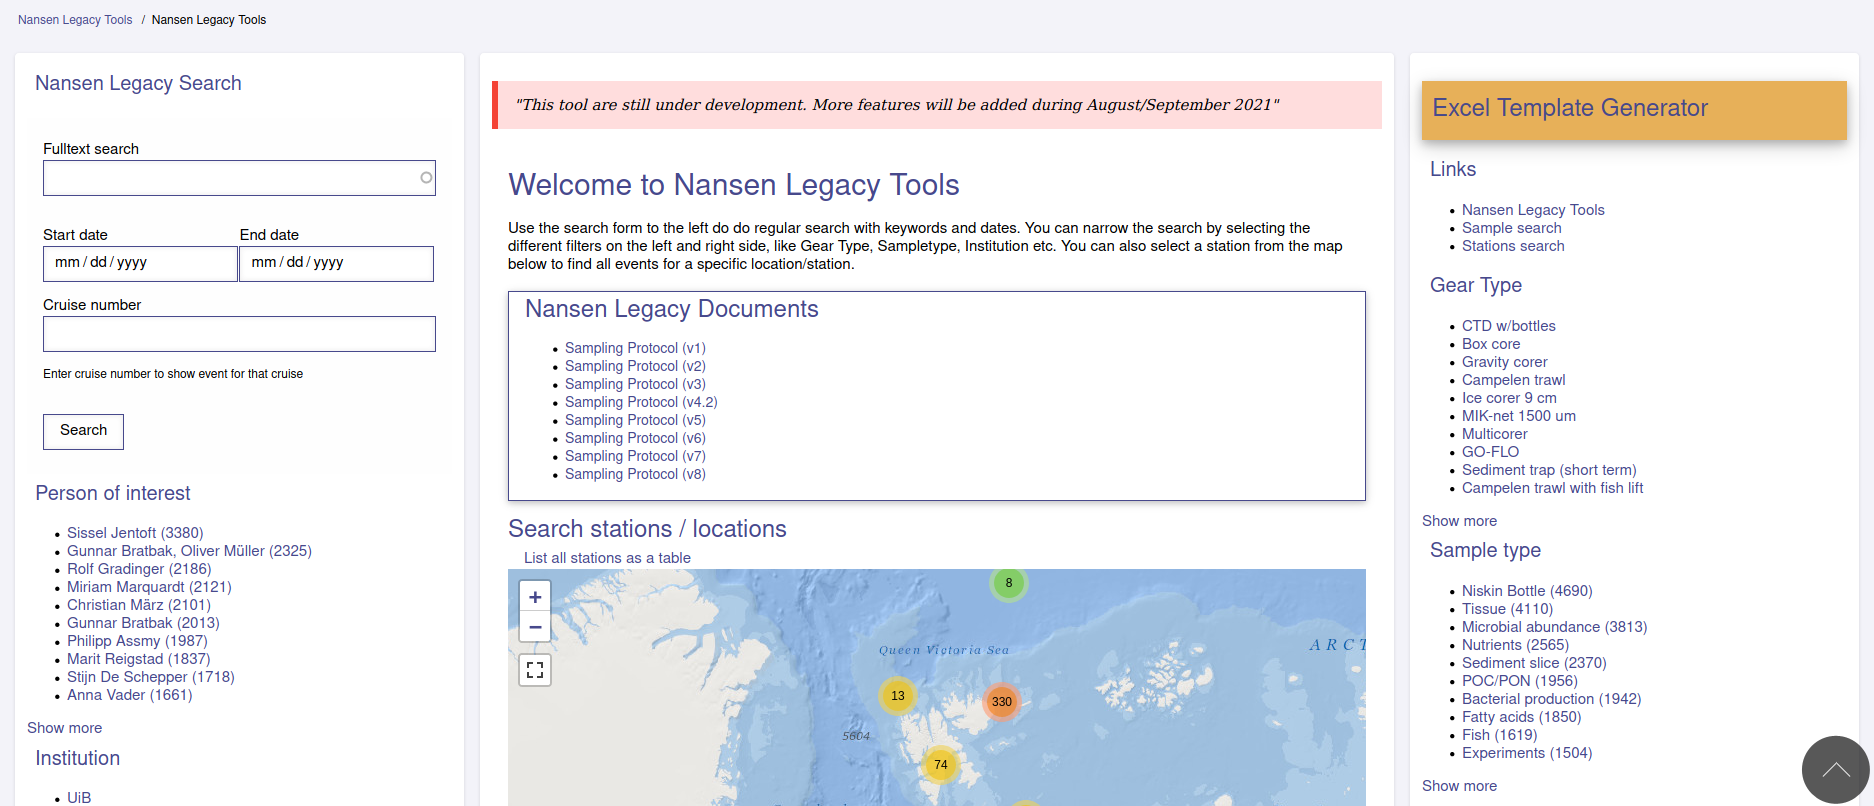
\includegraphics[width=0.7\textwidth]{SIOS_page}
    }
    \caption{\label{fig:sios}
        Top of page for sample log search at \url{https://sios-svalbard.org/reports/aen_multi}.
    }
\end{figure}
In the following subsection several scenarios will be explained. 

\subsection{Searching for individual samples} % (fold) {{{
\label{sub:search_ind}

If you know the ID of the sample you are interested in, you can use the \href{https://www.sios-svalbard.org/reports/ind_sample}{\color{blue}\underline{Sample ID search}} to find it. Input the ID in the search field by for instance scanning it and press "Search". If there is a sample with the given ID, all its information will be shown together with a map marking its location. At the bottom, a table of its children (if any) is shown. Clicking on different parts of the metadata will preform searches for samples with the same metadata. 

% subsection search_ind (end) }}}

\subsection{Find samples} % (fold) {{{
\label{sub:find_samples}

If you want to find samples based on location, time, cruise, gear type, sample type, parent event ID and/or station name, you want to use the \href{https://sios-svalbard.org/reports/aen_multi}{\color{blue}\underline{Sample Search}} page. Here you can choose one or more parameters to filter the database on. Make sure that you set the date range so it covers the times you are interested in (the first cruise in the Nansen Legacy was in June 2018).

After clicking search, a table of the results should be shown if there are any results. By clicking on the event ID, detailed information of the sample can be shown. If you want detailed information about all the returned samples, the easiest is to download it via the \emph{Get full information from the search as a tab separated file} link. This gives a tab separated file that can be opened in a spreadsheet viewer like Excel or Libre Office. 

\subsection{Samples from a given station} % (fold) {{{
\label{sub:station_search}

If you know the station name and want the samples from it, it is possible to use the \href{https://www.sios-svalbard.org/reports/aen_station}{\color{blue}\underline{Station Search}} page. Select the station and press search. It will show the location of the station on a map and its position, either as an average over all the samples taken from it or the defined position, if available. The samples taken at the station is shown in the table.

An overview over all the stations can be found using the \href{https://www.sios-svalbard.org/reports/aen_plot_all_stations}{\color{blue}\underline{Station Overview}} link.

% subsection station_search (end) }}}


\subsection{Search for multiple samples} % (fold) {{{
\label{sub:search_multi}
If you have an Excel sheet or a number of samples you want to get the (updated) information about, it is possible to use the multiple search interface. It takes space separated event IDs as an input. This can be inputted in the text box by pasting from a column in a spreadsheet (Excel) or repeatedly scanning codes with a scanner. 

After inputting all the codes, press \emph{Search}. If the IDs exist they should be displayed in a table. By pressing the export button all the information about them can be exported to a tab separated file.
% subsection search_multi (end) }}}

\subsection{Full sample log} % (fold) {{{
\label{sub:Full sample log}
A copy of the full sample log as a tab separated file can be downloaded using the \newline \href{https://www.sios-svalbard.org/cgi-bin/export_search.cgi?&startdate=2018-01-01&enddate=3000-01-01&geartype=&sampletype=&cruisenumber=&parenteventid=&startlat=&startlon=&endlat=&endlon=&stationname=}{\color{blue}\underline{Full sample log as CSV (without metadata)}} link.
% subsection Full sample log (end) }}}

% subsection find_samples (end) }}}



% section Searching_sample (end) }}}

\clearpage
\newpage
\appendix
\section*{Appendix}

\section{Technical details} % (fold) {{{
\label{sec:Technical details}

\subsection{UUID} % (fold) {{{
\label{sub:UUID}

A universally unique identifier (UUID) is a 32 character hex number, with 4 dashes splitting it into parts. An example is \emph{55702a3a-1ef4-11e9-b911-005056c00001}. It is a very common ID when one desires an identifier that is unique (on a global scale).

\subsubsection{Generation} % (fold) {{{
\label{ssub:Generation}

The reason for using UUIDs (universally unique identifier) to mark samples is that, given a good seed, the generation of UUIDs (with for example UUID1) ensures that the code is unique (the probability of collision is on the order of $ 2\times10^{-18}$). UUID1 contains the time and information about the computer generating it. It is a good code to use in the Nansen Legacy as the first 8 characters are sequential (time) and can be printed in clear text on the label to help with finding samples. UUID generation is implemented in most languages, and is easily done in for instance Python by importing the built in library \emph{uuid}. 

% subsection Generation (end) }}}

\subsubsection{Data Matrix} % (fold) {{{
\label{ssub:DM}
Samples are identified by UUIDs in the form of hex numbers, example \emph{388613ee-1a67-11e9-b5cc-a0481c9e7d26}. As these contain 36 characters, it is impractical to manually type these, therefore they are printed in the form of  Data Matrix (DM) codes following the ECC 200 standard. To fit the UUID, the DM code is of size $22\times22$, see figure~\ref{fig:data_matrix}. These DMs can be printed in different sizes and read by 2D barcode readers, webcameras and mobile phones. 


% subsection Data Matrix (end) }}}

\subsection{Printer} % (fold) {{{
\label{sub:Printer}
To ensure that the labels can be printed in the field and that the marking stays on, thermal transfer printers are used. One printer is available for each label size. In addition to printing the Data Matrix code, these printers are able to add information from each scientist in human readable format (text), helping to identify the sample without the need to scan it each time.

The chosen printer is a \emph{Zebra GX430t} printer. It was chosen as it puts few limitations on the labels used, and it can be printed used both from software and custom written Python software in the form of a web page. ZPL codes are used to specify what to print. These support Data Matrix codes following the ECC 200 standard.

% subsection Printer (end) }}}

In operation the printer uses ribbon, type \emph{Zebra 5095} which needs to periodically be changed, though this is not a large running cost.

\subsection{Scanner} % (fold) {{{
\label{sub:Scanner}

Data Matrix codes can be read with a smartphone or a webcamera, though this is not as fast as a dedicated scanner, but it is useful for scanning samples at home institutions. On the ship there are USB scanners available, which should be used to insert the UUID codes in the spreadsheet. They work like keyboards, place the cursor in the desired cell and press the scan button on the scanner.

There are two different types of scanners, the \emph{Opticon OPI-3601} and the \emph{Datalogic PowerScan PD9530-DPM}. Most scientists like the \emph{Opticon} best, but for environments with a lot of water the more expensive and waterproof \emph{Datalogic} is recommended.
% subsection Scanner (end) }}}

\subsection{Programs} % (fold) {{{
\label{sub:Programs}
The programs uses and their webpages are available through the SIOS GitHub page: \url{https://github.com/SIOS-Svalbard/}. They are written in mostly Python, PHP, JavaScript and PostgreSQL.
% subsection Programs (end) }}}

% section Technical details (end) }}}

%\section{List of equipment and costs} % (fold) {{{
%\label{sec:Costs}
%Table~\ref{tab:costs} shows the list of the different types of equipment and their approximate cost (on Svalbard). 
%\begin{table}[htb]
    %\rowcolors{3}{cyan!10}{white}
    %\caption{\label{tab:costs}List of equipment and unit costs. For the label if fewer labels are ordered, the unit price goes up. This is based on prices in 2018 to Svalbard, when this equipment was ordered.}
    %\begin{tabular}{lllr}
        %\hline
        %\textbf{Item} & \textbf{Product name} & \textbf{Unit size} & \textbf{Unit price} \\ \hline
        %Small label     & CILS 10 mm diam, 8100X  & Per label  (10 000)   & 0.74 NOK  \\ 
        %Medium label    & CILS Eppendorf, 81000TN & Per label  (20 000)   & 1.33 NOK  \\ 
        %Large label     & CILS, 8100X             & Per label  (10 000)   & 0.83 NOK  \\ 
        %Printer         & Zebra GX430t (GX43-102420-000)            & Per unit              & 5 397 NOK  \\ 
        %Printer ribbon  & Zebra 5095, 84 mm &     $ 12\times74$~m         & 640  NOK   \\ 
        %Opticon scanner & Opticon OPI-3601 USB    & Per unit              & 1 296 NOK  \\ 
        %Datalogic scanner & Datalogic PD9530-DPM  & Per unit              & 5 781 NOK  \\ 
        %\hline
    %\end{tabular}
%\end{table}


% section Costs (end) }}}

\end{document} 
